\documentclass{beamer}

\usepackage[T3]{fontenc}
\usepackage[utf8]{inputenc}
\usepackage[russian]{babel}

\usepackage{mhchem}
\usepackage{amssymb, amsmath}

%\usetheme{AnnArbor}
%\usetheme{Antibes}
%\usetheme{Bergen}
%\usetheme{Berkeley}
%\usetheme{Berlin}
%\usetheme{Boadilla}
%\usetheme{boxes}
%\usetheme{CambridgeUS}
%\usetheme{Copenhagen}
%\usetheme{Darmstadt}
%\usetheme{default}
%\usetheme{Frankfurt}
%\usetheme{Goettingen}
%\usetheme{Hannover}
%\usetheme{Ilmenau}
%\usetheme{JuanLesPins}
%\usetheme{Luebeck}
\usetheme{Madrid}
%\usetheme{Malmoe}
%\usetheme{Marburg}
%\usetheme{Montpellier}
%\usetheme{PaloAlto}
%\usetheme{Pittsburgh}
%\usetheme{Rochester}
%\usetheme{Singapore}
%\usetheme{Szeged}
%\usetheme{Warsaw}

\title{Отчет}

\author{Финенко Артем}

\institute[myuni] % (optional, but mostly needed)
{
  МГУ им. М.В.Ломоносова \\
  Химический факультет
}

\date{11/11/2016}

\pgfdeclareimage[height=0.5cm]{university-logo}{../pictures/logo.jpg}
\logo{\pgfuseimage{university-logo}}

% Let's get started
\begin{document}

\begin{frame}
  \titlepage
\end{frame}

\begin{frame}{Синтез 2-бензилиденциклопентанона}
\begin{block}{Схема реакции}
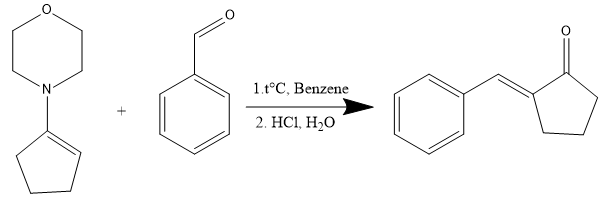
\includegraphics[scale=0.5]{../pictures/1.png}
\end{block}
\end{frame}

\begin{frame}{Синтез 2-бензилиден-5-(4-метоксибензилиден)циклопентанона.}
\begin{block}{Схема реакции}
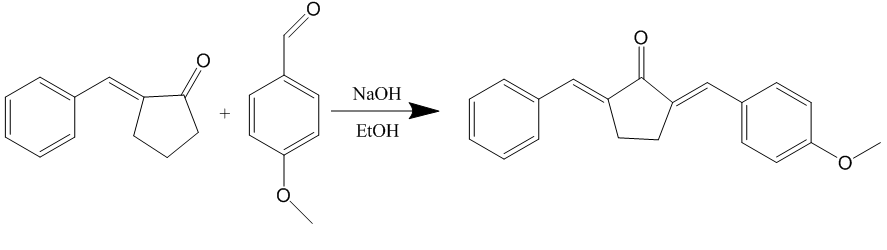
\includegraphics[scale=0.35]{../pictures/2.png}
\end{block}
\end{frame}

\begin{frame}{Синтез 2-бензилиден-5-(пиридин-3-илметилен)циклопентанона.}
\begin{block}{Схема реакции}
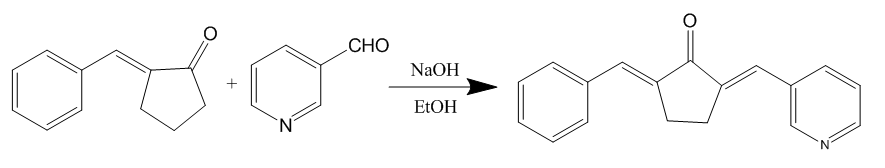
\includegraphics[scale=0.35]{../pictures/3.png}
\end{block}
\end{frame}

\begin{frame}{Синтез бензил-1,4-диил-диметилидендициклопентанона.}
\begin{block}{Схема реакции}
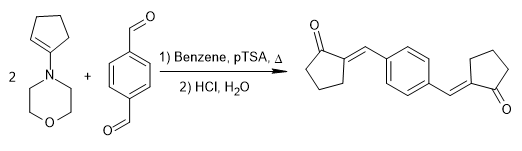
\includegraphics[scale=0.5]{../pictures/4.png}
\end{block}
\end{frame}

% All of the following is optional and typically not needed. 
\appendix
\section<presentation>*{\appendixname}
\subsection<presentation>*{For Further Reading}

\begin{frame}[allowframebreaks]
  \frametitle<presentation>{For Further Reading}
    
  \begin{thebibliography}{10}
    
  \beamertemplatebookbibitems
  % Start with overview books.

  \bibitem{Author1990}
    A.~Author.
    \newblock {\em Handbook of Everything}.
    \newblock Some Press, 1990.
 
  \bibitem{Someone2000}
    S.~Someone.
    \newblock On this and that.
    \newblock {\em Journal of This and That}, 2(1):50--100,
    2000.
  \end{thebibliography}
\end{frame}

\end{document}